\documentclass[12pt,letterpaper]{article}
\usepackage[margin=1in]{geometry}

\usepackage[utf8]{inputenc} % OJO!!!  => MANTENER ESTA LINEA PARA FACIL CONVERSION A WORD EN EL FUTURO ...
% \usepackage[spanish]{babel}
\usepackage{graphicx} 
\usepackage{array}
\usepackage{tabularx}
\usepackage{amssymb, amsmath}

% Paquetes extras ... 
\usepackage{subfigure}
\usepackage{color}
\definecolor{mygreen}{RGB}{28,172,0} % color values Red, Green, Blue
\definecolor{mylilas}{RGB}{170,55,241}

\usepackage{hyperref}
\usepackage{enumitem}

\usepackage{amsmath,amsfonts,amssymb,amsthm,cancel,icomma,nicefrac,mathrsfs,
            eurosym,verbatim,environ,ifthen,ifdraft,pdfpages,float,booktabs}
\allowdisplaybreaks[1] 

\usepackage{color}
\definecolor{lstgrey}{rgb}{0.95,0.95,0.95}
\usepackage{listings}
\lstset{language=Matlab,
       backgroundcolor=\color{lstgrey},
       frame=single,
       basicstyle=\footnotesize\ttfamily,
       captionpos=b,
       tabsize=2,
  }

\lstset{language=Matlab,%
  %basicstyle=\color{red},
  breaklines=true,%
  morekeywords={matlab2tikz},
  keywordstyle=\color{blue},%
  morekeywords=[2]{1}, keywordstyle=[2]{\color{black}},
  identifierstyle=\color{black},%
  stringstyle=\color{mylilas},
  commentstyle=\color{mygreen},%
  showstringspaces=false,%without this there will be a symbol in the places where there is a space
  numbers=left,%
  numberstyle={\tiny \color{black}},% size of the numbers
  numbersep=9pt, % this defines how far the numbers are from the text
  emph=[1]{for,end,break},emphstyle=[1]\color{red}, %some words to emphasise
  %emph=[2]{word1,word2}, emphstyle=[2]{style},    
}

\title{Asignment 1}
\author{Jose Eduardo Laruta Espejo \\ Facultad de Ingeniería - Universidad Mayor de San Andrés}
\begin{document}
\maketitle
\section{Problem 1}
\subsection{Matlab Code}

\lstinputlisting[label={lst:code1}, caption={Code for Problem 1}]{../matlab/ee6543_assignment1_problem1.m}

\subsection{Plots and Analysis}
From the code, the variable \verb|sigman1| represents the variance for the channel noise. This means that the greater 
this number, the harder to compensate its effects and this can be observed in the 
learning curve for both values. In the case of \verb|sigman1| being $10^{-5}$ 
the plots in Figure(\ref{fig:simu5}) show that the error converges at a lower value than when \verb|sigman1|
is $10^{-2}$. Another aspect is the variation or the \textit{jitter} present in both plots.

%%%% Figura 1 %%%%%%
\begin{figure}[!h] 
\centering
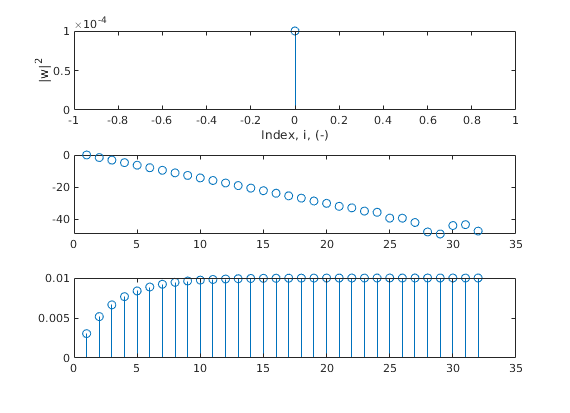
\includegraphics[width=0.8\textwidth]{../matlab/img/e-5.png}
\caption{plot for sigma1n=10e-5}
\label{fig:simu5}
\end{figure}

\begin{figure}[!h] 
    \centering
    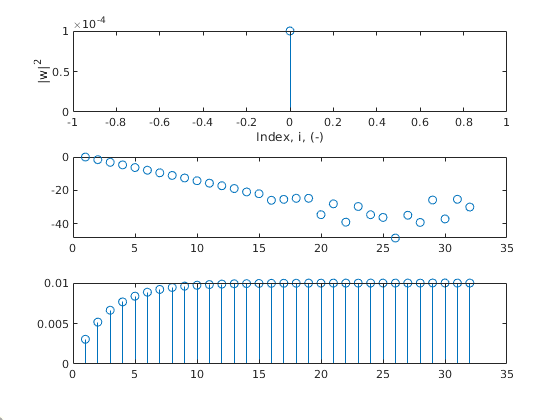
\includegraphics[width=0.8\textwidth]{../matlab/img/e-2.png}
    \caption{plot for sigma1n=10e-2}
    \label{fig:simu2}
\end{figure}
    

\section{Problem 2}
The learning curve flattens out even though there is no noise because the learning process has reached the minimum
value expressed by the wienner solution. This value corresponds to the minimum of the quadratic curve.

\begin{figure}[!h] 
  \centering
  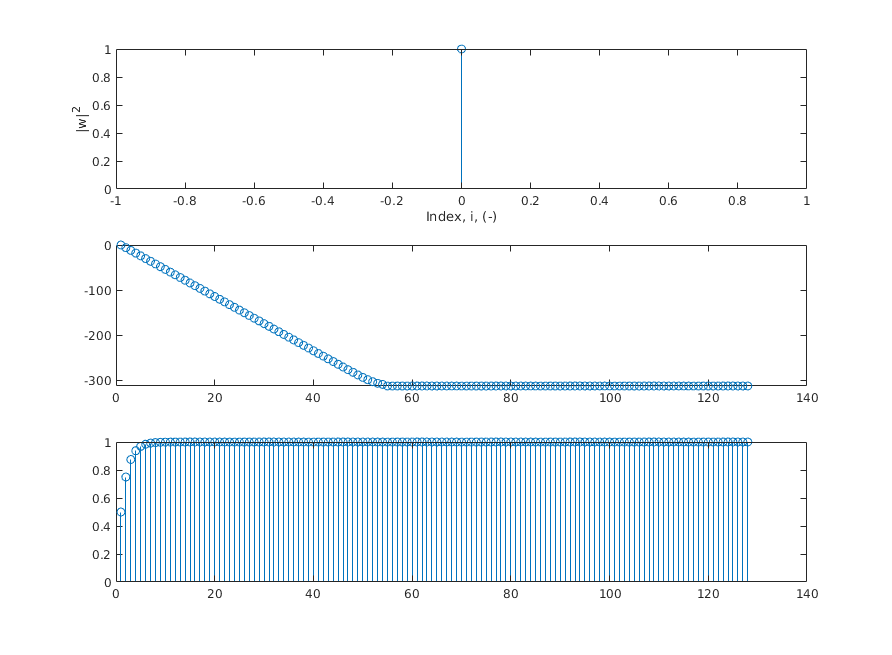
\includegraphics[width=0.8\textwidth]{../matlab/img/flat.png}
  \caption{plot without channel noise}
  \label{fig:flat}
\end{figure}

The value at which the learning curve (Fig \ref{fig:flat}) flattens is -313.1 dB, and its negative is 313.1 dB which corresponds with 
the SNR of this particular system.


\end{document}